\documentclass[UTF8]{article}
% 中文支持
\usepackage[UTF8]{ctex}	
% pdf调用 封面
\usepackage{pdfpages}
% color宏包
\usepackage{color}  
% 导入图片
\usepackage{caption}
\usepackage{graphicx, subfig}
% 防止图片乱跑
\usepackage{float}
% 支持数学符号
\usepackage{amsmath}
% 支持代码块
\usepackage{listings}
% pdf加入大纲
\usepackage{hyperref}
% 大纲去红框
\hypersetup{hidelinks,
	colorlinks=true,
	allcolors=black,
	pdfstartview=Fit,
	breaklinks=true
}

% 绘制三线表
\usepackage{booktabs}    
% 消除警告
\usepackage{lmodern}

% 设置页面的环境,a4纸张大小,左右上下边距信息
\usepackage[a4paper, left=31.8mm, right=31.8mm, top=25.4mm, bottom=25.4mm]{geometry}

% 代码块的基本设置
\lstset{
 columns=fixed,       
 numbers=left,                                        % 在左侧显示行号
 numberstyle=\tiny\color{gray},                       % 设定行号格式
 frame=none,                                          % 不显示背景边框
 backgroundcolor=\color[RGB]{245,245,244},            % 设定背景颜色
 keywordstyle=\color[RGB]{40,40,255},                 % 设定关键字颜色
 numberstyle=\footnotesize\color{darkgray},           
 commentstyle=\it\color[RGB]{0,96,96},                % 设置代码注释的格式
 stringstyle=\rmfamily\slshape\color[RGB]{128,0,0},   % 设置字符串格式
 showstringspaces=false,                              % 不显示字符串中的空格
 language=matlab,                                        % 设置语言
}

% \begin{titlepage}
% % 封面信息
% 
\includepdf[pages={1}]{cover.pdf}
% \end{titlepage}

% 生成目录
% \tableofcontents
% \cleardoublepage

% 导入图片
% \begin{figure}[H]
%     \centering % 居中 
%     % 图片文件的相对路径
%     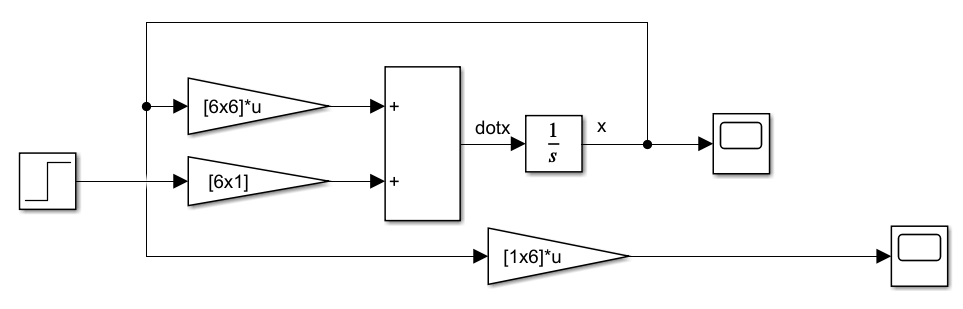
\includegraphics[width=.8\textwidth]{figure/exp1_1_model.png} 
%     \caption{Simulink模型} % caption是图片的标题
%     % \label{img} % 此处的label相当于一个图片的专属标志,目的是方便上下文的引用
% \end{figure}

% 导入代码
% \begin{lstlisting}
% a
% \end{lstlisting}

% 重置章节编号
% \setcounter{section}{0}

% \begin{table}[H] % 防止表格乱跑
% \centering % 居中
% \begin{tabular}{cccccc} % 指明列数
% 	\toprule % 顶部粗线
% 	序号 & 姓名 & 性别 & 年龄 & 身高/cm & 体重/kg \\
% 	\midrule % 中间细线
% 	1 & 张三 & M & 16 & 163 & 50 \\ % 每行末尾都要加换行符
% 	2 & 王红 & F & 15 & 159 & 47 \\
% 	3 & 李二 & M & 17 & 165 & 52 \\
% 	\bottomrule % 底部粗线
% \end{tabular}
% \caption{title} % 标题
% \end{table}

\begin{document}

\begin{titlepage}
% 封面信息

\includepdf[pages={1}]{./cover/cover.pdf}
\end{titlepage}

%
\section{工业控制网络的基本架构和组网原理}
% 进行关于 CAN 总线、ControlNet 网络组态等工业控制网络以及其对应的管理、组态软件的调研工作,学习工业控制网络的基本架构和组网原理。

% 选择任一现场总线或者工业以太网(可以是 CAN 总线也可以是其他总线或者网络),描述其网络的分层结构,进行网络控制或管理所使用的相关软件及其主要功能。

%%
\subsection{CAN总线}
%%%
\paragraph{CAN总线简介}~{}

CAN总线,全称为Controller Area Network,是ISO国际标准化的串行通信协议。这种总线是由德国以生产汽车电子产品而知名的BOSCH公司开发的,并最终成为了国际标准(ISO11519),是目前国际上应用最广泛的现场总线之一。

CAN总线属于现场总线的范畴,是一种有效支持分布式控制或实时控制的串行半双工通信网络。它分为低速和高速两种类型,低速CAN的传输速率为125kbps,高速CAN的传输速率可以达到1Mbps。此外,现在还有一种CAN FD,可以视为CAN的升级版,其传输速率更高。CAN总线因其高性能和可靠性,广泛应用于汽车、船舶等领域,用于连接汽车、船舶上的各个电子控制单元。

%%%
\paragraph{CAN总线的主要特点}~{}

在网络管理方面,基于CAN的网络管理(network management)是一种无中心式的网络管理,网络中的每个节点都依赖于自己和别人的通信状态来判断自己是处于睡眠状态还是唤醒状态。车载网络总线管理的目的是使网络中的ECU节点有序地睡眠和唤醒,在没有通信需求的时候睡眠,可以节约电池的能量。

此外,CAN总线的特点包括实时性强、传输距离较远、抗电磁干扰能力强、检错能力强,可在高噪声干扰环境中工作;具有优先权和仲裁功能,多个控制模块可以通过CAN控制器挂到CAN-bus上,形成多主机系统。总的来说,这些特点极大地提高了CAN总线的工作效率和稳定性,同时也增强了系统的可扩展性和可维护性。

%%
\subsection{CAN总线的网络控制、管理和组态软件及其主要功能}
CAN总线对应的网络控制、管理和组态软件主要有CANalyzer、CANape、CANopen等,它们主要负责对CAN总线上的设备进行监控和控制。下面对这些软件的主要功能分别进行介绍。

\begin{itemize}
	\item CANalyzer:用于 ECU 和网络的分析,解析汽车can报文,可收可发,可记录和回播报文。多用于汽车行业的开发和测试。CANalyzer是一款操作直观的综合软件工具,用于分析和模拟网络通信。使用 CANalyzer 检查网络上是否发生通信以及发生什么类型的通信;此外,除了发送或记录数据外,它还可以进行交互式 ECU 诊断。其特点包括操作直观、易于观察分析和补充数据流量、通过可配置的功能块(例如过滤器、交互式生成器或重放)实现灵活的分析功能、无缝记录总线数据并回放以进行离线分析、支持使用 CAPL 进行灵活编程,可用于广泛的分析任务等。
	\item CANape:CANape(CAN Application Programming Environment)是一款可用于ECU测量、标定、诊断以及ADAS传感器数据记录验证的综合性工具软件。工程师们通过CANape可以采集ECU数据,并对ECU信号进行可视化观测;可以优化ECU参数,而不需要修改程序代码,以调节ECU行为来适应各种车型;可以通过集成的诊断功能集实现对诊断数据和诊断服务的符号化访问。不仅如此,CANape还支持如雷达、激光雷达、摄像头等各类ADAS传感器数据采集,结合高性能硬件,每秒可以存储高达数千兆字节的数据。
	\item CANopen:CANopen组态软件是一款高性能又易用的工具,能够高效又直截了当地规划全部CANopen网络以及设备。它组合各种功能和直观操作性并在所有工程阶段给予支持,包括规划、开发、起步和服务。使用者能够马上集中精力到自己的应用和系统参数的定义上。CANopen组态软件包括CANopen DeviceExplorer、PDL (过程数据链接器)插件和独有的访问各种CAN接口的CAN驱动。

\end{itemize}

%%
\subsection{工业控制网络的基本架构和组网原理}
%%%
\paragraph{工业控制网络简介}~{}

工业控制网络是一种涉及局域网、广域网、分布式计算等多方面技术的网络,用于连接工业控制系统的工业计算机控制器、可编程逻辑控制器、传感器、变送器、执行器等设备。在工业自动化领域中,它还包含现场检测和控制系统。

%%%
\paragraph{基本架构}~{}

在工业生产控制过程中,工业控制系统负责具体的生产过程控制,工业控制网络则主要负责设备的连接和信息传输。工业控制网络的基本架构通常包括信息层、控制层和设备层,分别对应工业控制系统中的现场总线控制网络、过程控制与监控网络以及企业办公网络。信息层主要负责数据处理和传输,包括人机界面、生产管理信息系统等;控制层主要负责对生产过程进行监控和控制,包括PLC、DCS等;设备层则包括传感器、执行器等现场设备。

%%%
\paragraph{组网原理}~{}

工业控制网络的组网原理主要遵循“集中管理,分散控制”的原则。它连接各种设备节点,形成一个分布式的控制系统,实现数据的传输和共享,满足实时性、安全性、可扩展性和可靠性的要求。

相比使用流行的网络技术构建的信息网络,控制网络主要基于现场总线构建,对于通信的实时性和可靠性有着更高的要求。控制网络和信息网络通常紧密集成在一起,以建立统一的分布式数据库,保证所有数据完整性和互操作性。

此外,由于工业场景的多样性,工厂网络也呈现出多种特点。例如,为了确保高安全性、高稳定性和高可靠性,工厂网络经常需要进行网络隔离,即“专网专用”。同时,为了保证数据安全,许多工厂更倾向于对数据进行本地分离,在私有云设备/服务器上存储数据。

%
\section{工业控制网络的难点问题}
% 总结工业控制网络的难点是什么,当前有哪些解决措施或者方法。

目前工业控制网络面临的难点主要包括网络安全问题和网络体系结构的问题。

%%
\paragraph{网络安全问题}~{}

网络安全问题是工业控制网络目前面临的最主要的难点之一。随着我国进入工业转型的快速发展期,智能制造推动着信息化与工业化的不断融合,工业控制网络的安全问题日益突出。这主要表现在工厂缺乏网络技术常识和安全意识,以及工控网络安全的体系建设尚处于摸索和成长阶段,相关的标准和管理规定尚未完善。此外,随着越来越多的工业信息安全事件的出现,我国的工业基础设施正面临着前所未有的挑战。网络安全问题的具体表现如下:

\begin{enumerate}
	\item 工业控制系统自身安全性不强,当前主流的工业控制网络普遍存在安全漏洞,且多为能够造成远程攻击、越权执行的严重威胁类漏洞,近年来漏洞的数量呈快速增长的趋势,特别是SCADA、HMI、PLC、工业交换机等漏洞数量排名靠前。
	\item 工业控制网络通信协议的安全性问题,各控制系统厂商的私有通信协议在设计时侧重于实时性和可用性,缺乏对安全性的考量,如薄弱的加密算法和安全认证机制、不完善的授权权限等。协议的不安全性增加了网络层窃听、篡改、冒用攻击的吸引力。
	\item 在工业生产的实际环境中,存在大量老旧的系统和软件,并且系统补丁兼容性差,系统软件没有得到及时升级。
	\item 工业企业覆盖面广,细分行业众多,行业存在安全门槛。普遍认为进入电力行业的工控安全产品具有较高的标准和门槛,其他如能源、轨道交通、烟草、医药、制造业由于其业务应用场景不同,要基于其行业业务应用规则或工艺场景进行安全防护;同时各工业企业信息安全水平不一而足,差距明显。
	\item 来自外部网络环境的威胁经常出现,针对工业控制系统的网络攻击事件频发。国家层面的网络空间安全博弈、利用信息和通信技术进行的致命性攻击以及对国家重要基础设施对象和相关信息系统的攻击愈加严峻。
\end{enumerate}

为了解决这些问题,当前采取的主要措施或方法包括加强基础网络安全建设,如部署Web应用防火墙等网络安全产品;提升技术人员的网络安全意识和技能;以及不断优化和完善工控安全的体系结构和相关管理规定。同时,也需要考虑到工业控制网络的特性和需求,以确保工业控制网络的稳定性和可靠性。

%%
\paragraph{网络体系结构问题}~{}

关于体系结构的问题。目前对于工业控制网络体系结构还没有形成统一的模式,这无疑增加了工业控制网络的设计和实施难度。工业控制网络体系结构目前面临着诸多挑战,包括:

\begin{enumerate}
	\item 传统架构的问题:传统的工业自动化封闭式五层架构已经不能满足现代工业生产的需求。这种架构不支持数据高效流转,限制了工业互联网的发展。
	\item 新技术的融合与标准化:随着信息技术和操作技术的深度融合,如TSN、工业软件定义网络(SDN)、确定性网络和智能网络管理等新技术领域的发展,对标准化的需求也在不断涌现。而现有的工业互联网总体现状和顶层设计标准仍需进一步完善。
	\item 企业网络化与信息化的挑战:随着工业企业网络化、信息化进程的不断推进,如何将生产管控、物料管理、事务处理等多种业务流程整合为信息资源,同时确保网络安全和稳定性,是当前的主要挑战。
	\item 网络协同与控制功能虚拟化:现代工业控制网络需要支持更加灵活的任务部署和控制功能虚拟化。例如,CaaS技术可以将整个工业控制网络虚拟为一个通用控制器,支持生产线的灵活切换与升级。
	\item 无线网络的需求:随着“5G+工业互联网”的融合创新,工业智能化发展对无线网络的需求也在增加,特别是对大带宽、低时延、大连接特点的无线网络基础设施的需求。
\end{enumerate}

为了应对上述挑战,工业控制网络体系结构需要不断创新和完善,充分发挥新一代信息技术的赋能效应,提升制造业的高端化、智能化和绿色化发展水平。

%
\section{工业控制网络的发展趋势}
% 通过调研,总结工业控制网络今后的发展趋势。

经过调研和分析认为,工业控制网络今后可能的发展趋势有如下要点:

\begin{enumerate}
	\item 工业互联网的发展:随着工业4.0的到来,工业互联网将成为工业控制网络的重要发展方向。通过将工业设备、生产线、工厂等连接在一起,实现设备的远程监控、故障预警、智能维护等功能,提高生产效率和质量。
	\item 5G技术的应用:5G技术的高速度、低延迟、大连接数等特点,将为工业控制网络带来革命性的变化。通过5G技术,可以实现设备之间的高速通信,提高生产协同效率;同时,5G技术还可以支持更多的传感器和设备接入,实现更精细化的生产管理。
	\item 边缘计算的普及:随着物联网设备的大量增加,数据处理的压力也在不断增大。边缘计算可以将数据处理任务分散到设备附近的边缘节点上,降低数据传输的延迟和成本,提高数据处理的效率。在工业控制网络中,边缘计算可以用于实时数据分析、设备状态监测等场景。
	\item 安全性的提升:随着工业控制系统对网络安全的重视程度不断提高,工业控制网络的安全性也将得到加强。未来,工业控制网络将采用更严格的加密技术、身份认证机制等手段,保障数据的安全传输和存储。
	\item 人工智能与机器学习的应用:人工智能和机器学习技术的发展,将为工业控制网络带来更多的创新应用。通过对大量数据的分析和挖掘,可以实现生产过程的优化、设备的智能调度等功能,提高生产效率和降低成本。
	\item 开放性和标准化:为了实现不同厂商设备之间的互操作性,工业控制网络将更加注重开放性和标准化。通过制定统一的通信协议、接口标准等,降低设备集成的难度,促进产业链的协同发展。
\end{enumerate}

%
\section{典型应用:工业控制网络在汽车制造行业的应用}
% 详细描述一个工业控制网络的典型应用。以某一行业,例如汽车制造、钢铁生产等工业生产领域的应用为例子,说明该应用中采用的工业控制网络的结构、网络性能、特点等。

汽车制造是一个高度自动化的生产过程,涉及到大量的机械、电气和电子系统。为了实现这些系统的高效协同工作,汽车制造商通常采用工业控制网络来连接和管理这些设备。

%% 
\paragraph{结构}~{}

在汽车制造过程中,工业控制网络通常采用分层的结构,包括现场层、控制层和信息管理层。现场层主要包括各种传感器、执行器等设备,用于收集生产过程中的数据并将其传输到控制层。控制层主要由PLC(可编程逻辑控制器)和DCS(分布式控制系统)组成,负责对现场层设备进行实时监控和控制。信息管理层则包括MES(制造执行系统)和ERP(企业资源规划)等软件系统,用于处理和分析生产数据,为生产过程提供决策支持。

%% 
\paragraph{网络性能}~{}

汽车制造行业的工业控制网络需要具备高可靠性、实时性和安全性。为了实现这些性能要求,工业控制网络通常采用冗余设计和专用通信协议。例如,现场层设备可以通过以太网或Profinet等通信协议与控制层设备进行通信,而控制层设备则可以通过Modbus或EtherCAT等专用协议与信息管理层软件进行通信。此外,工业控制网络还需要具备一定的扩展性,以便在未来生产过程中根据需要增加新的设备和功能。

%% 
\paragraph{主要特点}~{}

汽车制造行业的工业控制网络具有以下特点:

\begin{itemize}
	\item 实时性:由于汽车制造过程涉及到大量的机械和电气系统,因此工业控制网络需要具备实时性,以确保生产过程的顺利进行。
	\item 可靠性:汽车制造过程中的任何故障都可能导致生产线的停滞,甚至造成严重的经济损失。因此,工业控制网络需要具备高可靠性,确保在各种异常情况下仍能正常工作。
	\item 安全性:汽车制造过程中涉及到大量的敏感数据,如生产工艺的过程数据等。因此,工业控制网络需要具备一定的安全性,防止数据泄露或被恶意篡改。
	\item 易用性:为了降低操作和维护成本,工业控制网络需要具备良好的易用性,使得工程师和操作人员能够快速地掌握其使用方法。
\end{itemize}

总之,汽车制造行业的工业控制网络通过采用分层结构、专用通信协议和冗余设计等技术手段,实现了高可靠性、实时性和安全性等性能要求。同时,工业控制网络还具备良好的易用性,为汽车制造过程提供了强大的支持。

\begin{thebibliography}{99}  
	\bibitem{ref1} 《现场总线技术及应用教程(第二版)》,王永华,机械工业出版社

	\bibitem{ref2} 《现场总线及工业控制网络》,汤旻安,机械工业出版社

	\bibitem{ref3} 《工业网络技术》,汪晋宽,北京邮电大学出版社

	\bibitem{ref4} \href{https://www.vector.com/int/en/products/products-a-z/software/canalyzer/#}{CANalyzer}:https://www.vector.com/int/en/products/products-a-z/software/canalyzer

	\bibitem{ref5} \href{https://www.hkaco.com/zdh/systec/industrial-communication/can-and-canopen/canopen-configuration-suite.html}{CANopen Configuration Suite - CANopen组态软件}:https://www.hkaco.com/zdh/systec/industrial-communication/can-and-canopen/canopen-configuration-suite.html

	\bibitem{ref6} \href{https://www.cnblogs.com/yaoyaojcy/p/9304209.html}{自学工业控制网络之路}:https://www.cnblogs.com/yaoyaojcy/p/9304209.html

	\bibitem{ref7} \href{https://zhuanlan.zhihu.com/p/138031445}{以太网、Profinet、Profibus三种网络架构搭建及拓扑分析 - 智能制造之家的文章 - 知乎}:https://zhuanlan.zhihu.com/p/138031445

	\bibitem{ref8} \href{https://blog.csdn.net/weixin_45263626/article/details/107893997}{工业控制网络概述}:https://blog.csdn.net/weixin\_45263626/article/details/107893997

	\bibitem{ref9} \href{https://www.jianshu.com/p/26200a6c0715}{工业控制网络}:https://www.jianshu.com/p/26200a6c0715

	\bibitem{ref10} \href{https://zhuanlan.zhihu.com/p/179076975}{工业控制系统的网络安全现状及改进方式 - 葫芦娃集团的文章 - 知乎}:https://zhuanlan.zhihu.com/p/179076975

	\bibitem{ref11} \href{https://zhuanlan.zhihu.com/p/116614311}{工业控制系统信息安全面临的紧迫问题分析 - 星河安全的文章 - 知乎}:https://zhuanlan.zhihu.com/p/116614311
	
	\bibitem{ref12} \href{https://www.zhihu.com/question/324431252/answer/2309246161}{商用密码应用安全性评估:工业控制网络的发展概况及趋势如何? - 沃通SSL证书的回答 - 知乎}:https://www.zhihu.com/question/324431252/answer/2309246161

	\bibitem{ref13} \href{https://www.elecfans.com/kongzhijishu/1080520.html}{工业控制系统未来的发展趋势分析}:https://www.elecfans.com/kongzhijishu/1080520.html

	\bibitem{ref14} \href{https://www.zhihu.com/question/324431252/answer/2697534315}{工业控制网络的发展概况及趋势如何? - 虚拟人生的回答 - 知乎}:https://www.zhihu.com/question/324431252/answer/2697534315

\end{thebibliography}

\end{document}